\documentclass{article}
\usepackage{graphicx} % Required for inserting images
\usepackage[UTF8]{ctex}
\usepackage[a4paper,left=10mm,right=10mm,top=15mm,bottom=15mm]{geometry}

\title{提问的智慧}
\author{Spike}
\date{October 2023}


\begin{document}

\maketitle
\renewcommand{\contentsname}{目录}
\tableofcontents

\begin{abstract}
    第一次使用latex记笔记,这是摘要
\end{abstract}
\newpage
%第一章
\section{使问题高效}
\subsection{思考问题、自主寻找信息}
\begin{figure}[h]
    \centering
    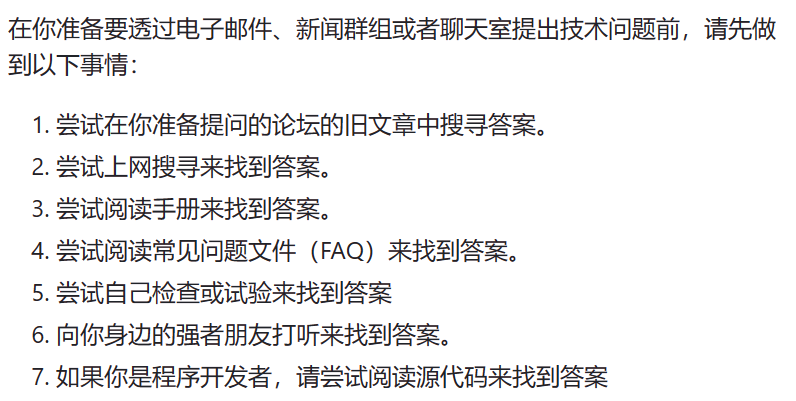
\includegraphics[width=18cm]{image_1.png}
    \caption{Try before u ask}
    \label{fig:enter-label}
\end{figure}

\subsection{注意场合}
明确问题涉及领域  确认提问平台/对象

\begin{figure}[h]
    \centering
    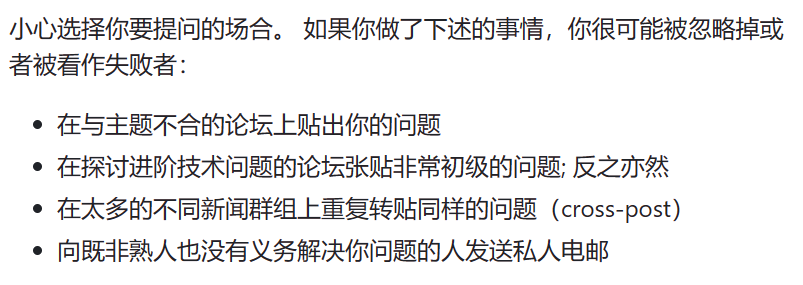
\includegraphics[width=18cm]{image_2.png}
    \caption{Station}
    \label{fig:enter-label}
\end{figure}

\newpage

\subsection{网络提问平台}

提问对象   其他用户(无果)→开发者列表

\subsubsection{Stack Exchange}
\begin{figure}[h]
    \centering
    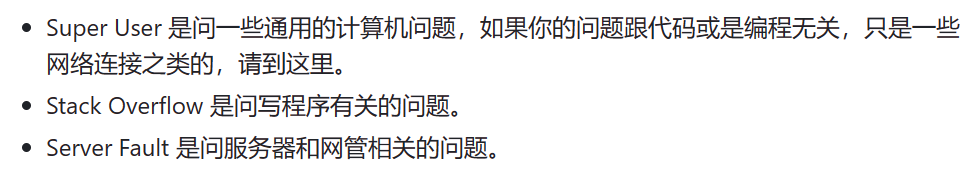
\includegraphics[width=18cm]{image3.png}
    \caption{Stack Exchange}
    \label{fig:enter-label}
\end{figure}

\subsubsection{IRC频道}
\begin{figure}[h]
    \centering
    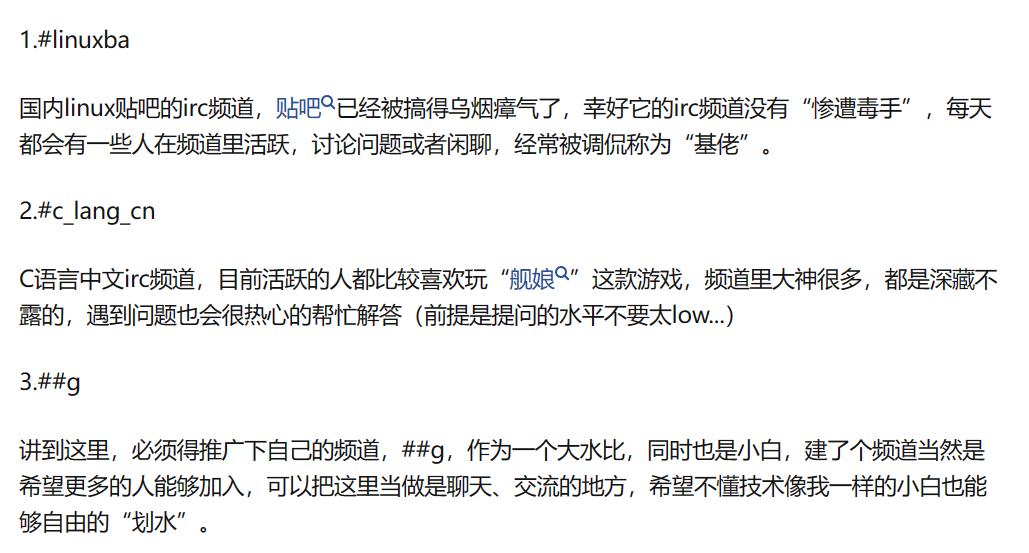
\includegraphics[width=18cm]{image6.png}
    \caption{IRC}
    \label{fig:enter-label}
\end{figure}
\newpage

\subsection{使用有意义且描述明确的标题(客观)}
\begin{figure}[h]
    \centering
    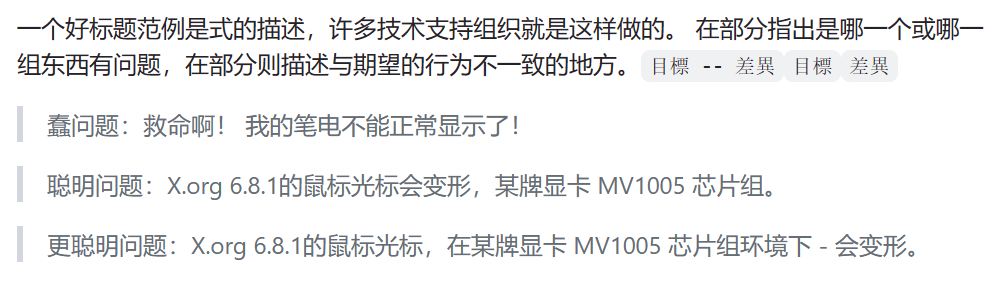
\includegraphics[width=18cm]{image4.png}
    \caption{IRC}
    \label{fig:enter-label}
\end{figure}

\subsection{使用  清晰  精准 的语句}
·若不确定语言,使用英语,标注语法问题\\
·确定自己的问题逻辑,所涉及的知识尽量不出错\\
·提供好的回答渠道、问题引流(网络论坛)\\
·好的文本输入习惯\\
\begin{figure}[h]
    \centering
    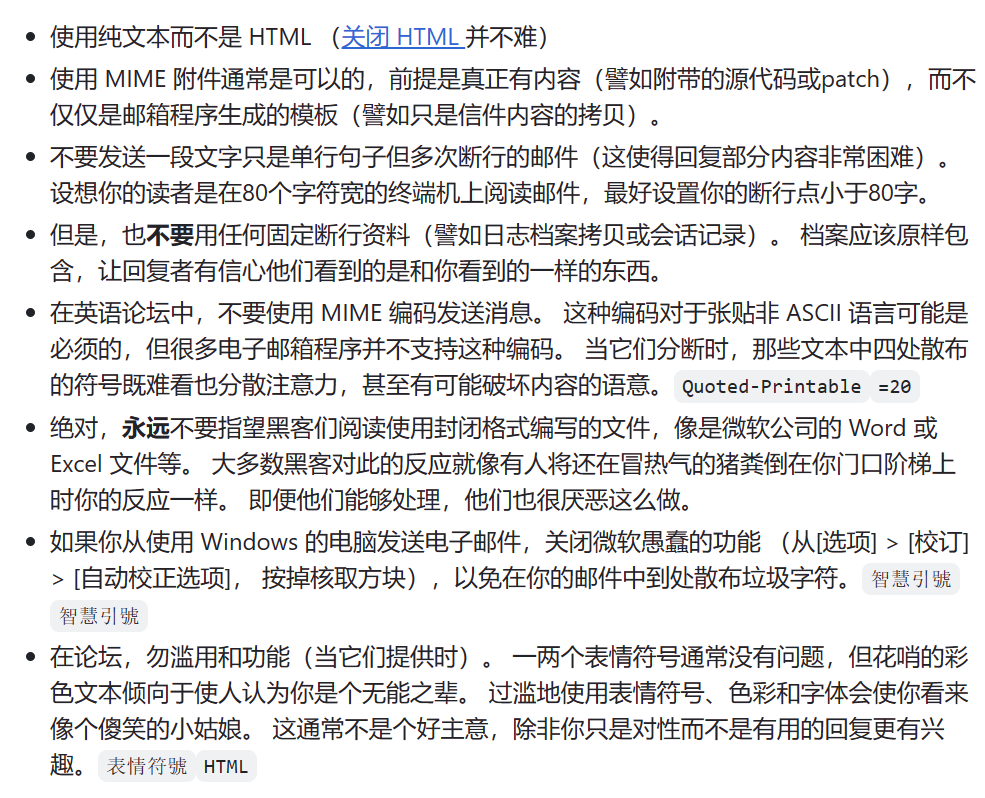
\includegraphics[width=11cm]{image5.png}
    \label{fig:enter-label}
\end{figure}

不要轻易表达自己的“猜测”以及“主观情绪”\\
  清晰描述自己希望达成的目标或是需求\\
  使问答公开、透明\\
  去除无意义的提问\\
!不贴作业!

\section{处理回答}
 \subsection{先弄清楚dalao提供的回答} 
      if  解决了问题→相关帖子中阐述解决方法,表达感谢
      else  至少表示出你从中学到了什么
\subsection{如果有无礼的回应}
  无需受负面情绪影响,平淡略过
  \subsection{如何回答问题}
  \begin{figure}[h]
    \centering
    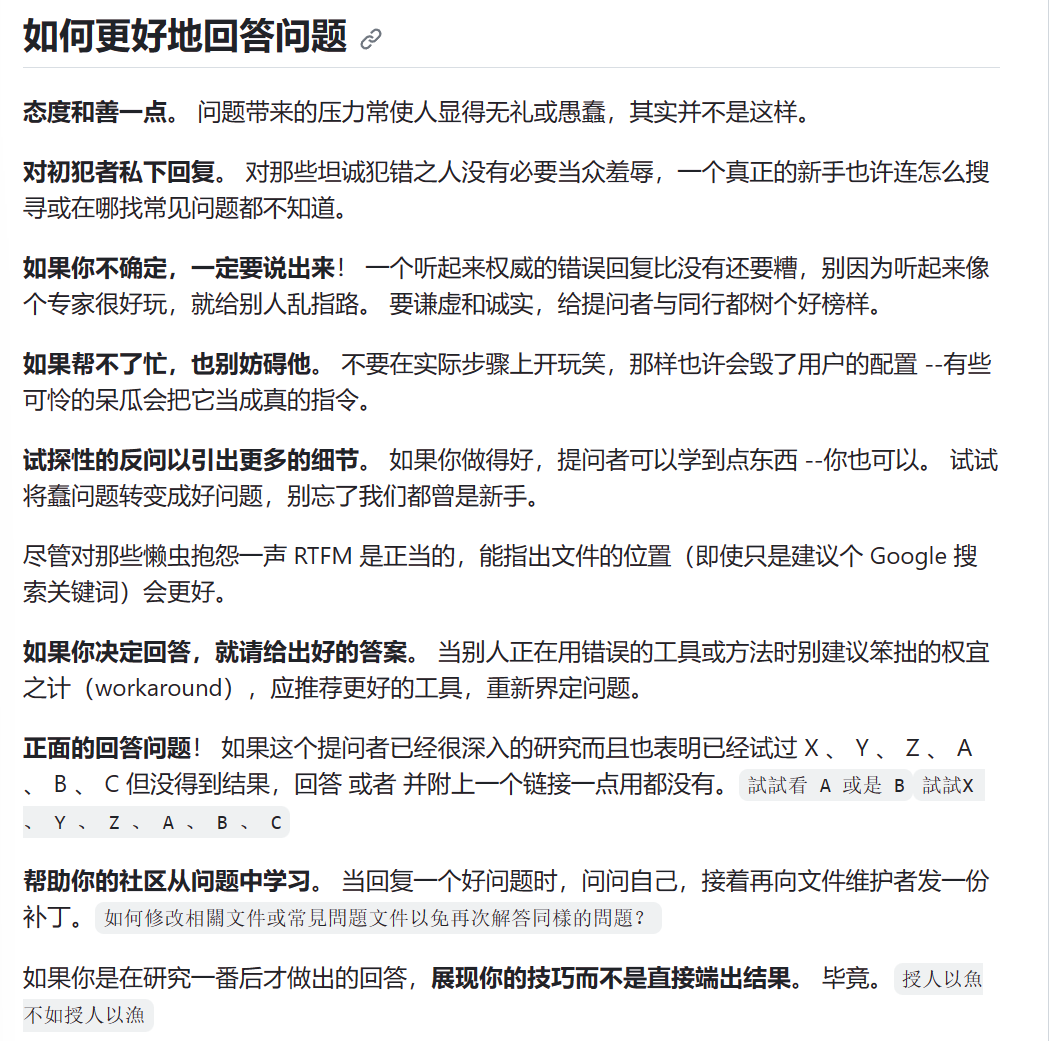
\includegraphics[width=18cm]{image7.png}
    \caption{回答问题}
    \label{fig:enter-label}
\end{figure}
  



\end{document}
